\documentclass[11pt, oneside]{article}
\usepackage[letterpaper, margin=2cm]{geometry}
\usepackage{MATH667}

\begin{document}
\noindent \textbf{\Large{Caleb Logemann \\
MATH667 Hyperbolic Partial Differential Equations
Homework 1
}}

%\lstinputlisting[language=MATLAB]{H01_23.m}
\begin{enumerate}
  \item % #1 Done
    For constant coefficient linear wave equation initial value problem
    \[
      \begin{cases}
        u_t + a u_x = 0 \\
        u(x, 0) = u_0(x)
      \end{cases}
    \]
    for all $x \in \RR$ and $t \ge 0$, verify that the solution
    $u(x, t) = u_0(x - at)$ satisfies the following integral form.
    We assume the initial $u_0(x)$ is a smooth function.
    \[
      \dintt{x_1}{x_2}{u(x, t_2)}{x} = \dintt{x_1}{x_2}{u(x, t_1)}{x} +
      \dintt{t_1}{t_2}{au(x_1, t)}{t} - \dintt{t_1}{t_2}{au(x_2, t)}{t}, \quad
      \forall x_1, x_2 \in \RR, \forall t_1, t_2 \ge 0.
    \]

    Let $U$ be an antiderivative of $u_0$, that is
    $\dintt{y_1}{y_2}{u_0(y)}{y} = U(y_2) - U(y_1)$.
    This is guaranteed to exist since $u_0$ is a smooth function.
    Now we can consider each of the terms of the integral form seperately.
    The first term can be simplified as follows,
    \begin{align*}
      \dintt{x_1}{x_2}{u(x, t_2)}{x} &= \dintt{x_1}{x_2}{u_0(x - at_2)}{x} \\
      &= U(x_2 - at_2) - U(x_1 - at_2).
    \end{align*}
    The second term is
    \begin{align*}
      \dintt{x_1}{x_2}{u(x, t_1)}{x} &= \dintt{x_1}{x_2}{u_0(x - at_1)}{x} \\
      &= U(x_2 - at_1) - U(x_1 - at_1).
    \end{align*}
    The third term is
    \begin{align*}
      \dintt{t_1}{t_2}{au(x_1, t)}{t} &= \dintt{t_1}{t_2}{au_0(x_1 - at)}{t} \\
      &= \frac{a}{-a} \p{U(x_1 - at_2) - U(x_1 - at_1)} \\
      &= - U(x_1 - at_2) + U(x_1 - at_1).
    \end{align*}
    The last term becomes
    \begin{align*}
      \dintt{t_1}{t_2}{au(x_2, t)}{t} &= \dintt{t_1}{t_2}{au_0(x_2 - at)}{t} \\
      &= \frac{a}{-a} \p{U(x_1 - at_2) - U(x_1 - at_1)} \\
      &= -U(x_2 - at_2) + U(x_2 - at_1).
    \end{align*}

    Combining these four terms back into the integral form gives.
    \begin{align*}
      U(x_2 - at_2) - U(x_1 - at_2) &= U(x_2 - at_1) - U(x_1 - at_1) - U(x_1 - at_2) \\
        &+ U(x_1 - at_1) + U(x_2 - at_2) - U(x_2 - at_1) \\
      U(x_2 - at_2) - U(x_1 - at_2) &= - U(x_1 - at_2) + U(x_2 - at_2) \\
      - U(x_1 - at_2) &= - U(x_1 - at_2)  \\
      0 &= 0
    \end{align*}
    This shows that the integral form is satisfied for all values of $x_1, x_2 \in \RR$ and $t_1, t_2 \ge 0$.

  \item % #2 Done
    For viscous Burger's equation $u_t + uu_x + \varepsilon u_{xx}$ with initial condition
    \[
      u(x, 0) =
      \begin{cases}
        1 & x \le 0 \\
        0 & x > 0
      \end{cases},
    \]
    verify the traveling wave solution $u_{\varepsilon}(x, t)$ satisfies the given PDE.\@
    We have $u_{\varepsilon}(x, t) = w(x - \frac{1}{2}t)$, where
    $w(y) = \frac{1}{2}\p{1 - \tanh{\frac{y}{4\varepsilon}}}$.
    Graph the solution $u_{\varepsilon}(x, t)$ at $t = 1$ with
    $\varepsilon = 10^{-2}, 10^{-4}, 10^{-6}$.

    First note that
    \begin{align*}
      u_{\varepsilon, t} &= -\frac{1}{2} w'\p{x - \frac{1}{2}t} \\
      u_{\varepsilon, x} &= w'\p{x - \frac{1}{2}t} \\
      u_{\varepsilon, xx} &= w''\p{x - \frac{1}{2}t}.
    \end{align*}
    Also note the derivatives of $w$ are
    \begin{align*}
      w'(y) = -\frac{1}{8\varepsilon} \p{1 - \tanh[2]{\frac{y}{4\varepsilon}}} \\
      w''(y) = \frac{1}{16\varepsilon^2} \tanh{\frac{y}{4\varepsilon}} \p{1 - \tanh[2]{\frac{y}{4\varepsilon}}} \\
    \end{align*}
    Now we see that
    \begin{align*}
      u_{\varepsilon, t} &= \frac{1}{16\varepsilon} \p{1 - \tanh[2]{\frac{x - \frac{1}{2}t}{4\varepsilon}}}\\
      u_{\varepsilon, x} &= -\frac{1}{8\varepsilon} \p{1 - \tanh[2]{\frac{x - \frac{1}{2}t}{4\varepsilon}}} \\
      u_{\varepsilon, xx} &= \frac{1}{16\varepsilon^2} \tanh{\frac{x - \frac{1}{2}t}{4\varepsilon}} \p{1 - \tanh[2]{\frac{x - \frac{1}{2}t}{4\varepsilon}}}.
    \end{align*}
    Plugging these into the left hand side and right hand side of the PDE gives the following.
    First I will simplify the left hand side
    \begin{gather*}
      u_{\varepsilon, t} + u_{\varepsilon} u_{\varepsilon, x} \\
      \frac{1}{16\varepsilon} \p{1 - \tanh[2]{\frac{x - \frac{1}{2}t}{4\varepsilon}}} + -\frac{1}{2}\p{1 - \tanh{\frac{x - \frac{1}{2}t}{4\varepsilon}}}\frac{1}{8\varepsilon} \p{1 - \tanh[2]{\frac{x - \frac{1}{2}t}{4\varepsilon}}} \\
      \frac{1}{16\varepsilon} - \frac{1}{16\varepsilon}\tanh[2]{\frac{x - \frac{1}{2}t}{4\varepsilon}} + \p{-\frac{1}{16\varepsilon} + \frac{1}{16\varepsilon}\tanh{\frac{x - \frac{1}{2}t}{4\varepsilon}}} \p{1 - \tanh[2]{\frac{x - \frac{1}{2}t}{4\varepsilon}}} \\
      \frac{1}{16\varepsilon} - \frac{1}{16\varepsilon}\tanh[2]{\frac{x - \frac{1}{2}t}{4\varepsilon}} + -\frac{1}{16\varepsilon} + \frac{1}{16\varepsilon}\tanh{\frac{x - \frac{1}{2}t}{4\varepsilon}} + \frac{1}{16\varepsilon}\tanh[2]{\frac{x - \frac{1}{2}t}{4\varepsilon}} - \frac{1}{16\varepsilon}\tanh[3]{\frac{x - \frac{1}{2}t}{4\varepsilon}} \\
      \frac{1}{16\varepsilon}\tanh{\frac{x - \frac{1}{2}t}{4\varepsilon}} - \frac{1}{16\varepsilon}\tanh[3]{\frac{x - \frac{1}{2}t}{4\varepsilon}}.
    \end{gather*}
    Next I will simplify the right hand side
    \begin{gather}
      \varepsilon u_{\varepsilon, xx} \\
      \varepsilon \frac{1}{16\varepsilon^2} \tanh{\frac{x - \frac{1}{2}t}{4\varepsilon}} \p{1 - \tanh[2]{\frac{x - \frac{1}{2}t}{4\varepsilon}}} \\
      \frac{1}{16\varepsilon} \p{\tanh{\frac{x - \frac{1}{2}t}{4\varepsilon}} - \tanh[3]{\frac{x - \frac{1}{2}t}{4\varepsilon}}} \\
    \end{gather}
    We see that this is equal to the left hand side shown previously, so $u_{\varepsilon}(x, t)$ does satisfy the PDE.\@

    Also $u_{\varepsilon}(x, t)$ satisfies the inital conditions as $\varepsilon \to 0$.
    To see this consider the following
    \begin{align*}
      \lim[\varepsilon \to 0]{u_{\varepsilon}(x, 0)} &= \lim[\varepsilon \to 0]{\frac{1}{2}\p{1 - \tanh{\frac{x}{3\varepsilon}}}} \\
      &= \frac{1}{2} - \lim[\varepsilon \to 0]{\tanh{\frac{x}{4\varepsilon}}}
      \intertext{If $x \le 0$, then this is equivalent to}
      &= \frac{1}{2} - \lim[y \to -\infty]{\tanh{y}} \\
      &= \frac{1}{2} - -\frac{1}{2} = 1
      \intertext{If $x > 0$, then this limit is equivalent to}
      &= \frac{1}{2} - \lim[y \to \infty]{\tanh{y}} \\
      &= \frac{1}{2} - \frac{1}{2} = 0
    \end{align*}
    This shows that $u_{\varepsilon}(x, t)$ satisfies the initial conditions as $\varepsilon \to 0$.

    The following is a graph of $u_{\varepsilon}(x, 1)$ with $\varepsilon = 10^{-2}, 10^{-4}, 10^{-6}$.
    Note that graph for $\varepsilon = 10^{-4}$ and the graph for
    $\varepsilon = 10^{-6}$ are almost directly on top of on another.
    \begin{center}
      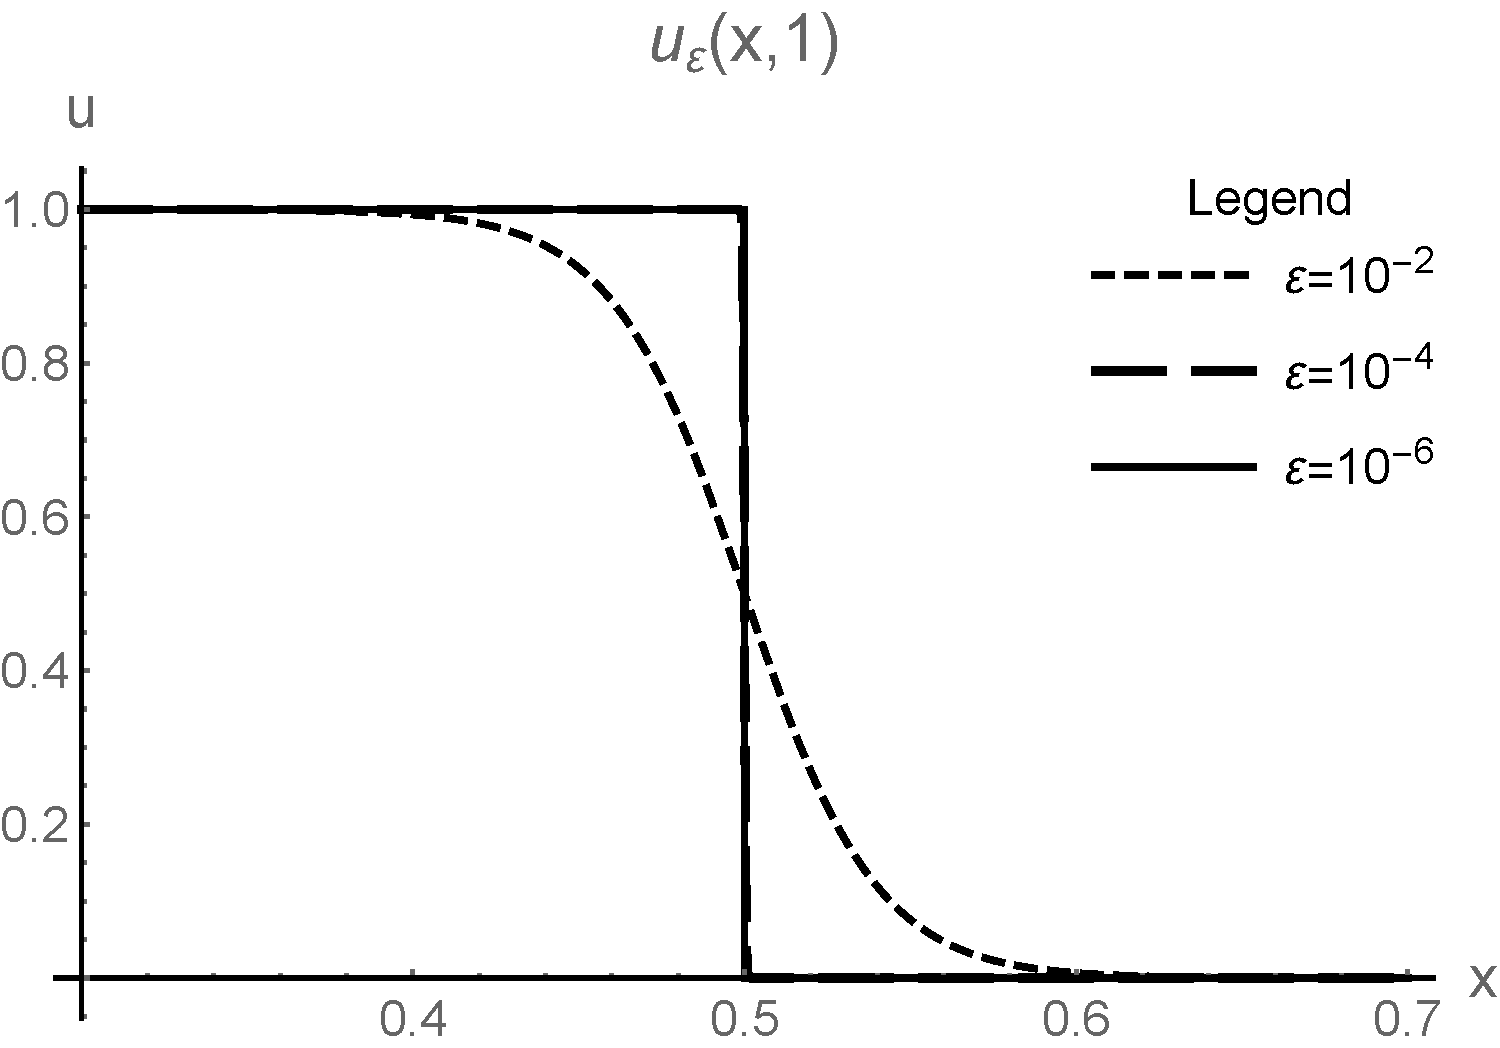
\includegraphics[scale=.5]{Figures/01_01}
    \end{center}

  \item % #3
    For Burger's equation Riemann problem $u(x, 0) = $

  \item % #4
\end{enumerate}
\end{document}
